% Options for packages loaded elsewhere
\PassOptionsToPackage{unicode}{hyperref}
\PassOptionsToPackage{hyphens}{url}
\PassOptionsToPackage{dvipsnames,svgnames,x11names}{xcolor}
%
\documentclass[
  letterpaper,
  DIV=11,
  numbers=noendperiod]{scrartcl}

\usepackage{amsmath,amssymb}
\usepackage{lmodern}
\usepackage{iftex}
\ifPDFTeX
  \usepackage[T1]{fontenc}
  \usepackage[utf8]{inputenc}
  \usepackage{textcomp} % provide euro and other symbols
\else % if luatex or xetex
  \usepackage{unicode-math}
  \defaultfontfeatures{Scale=MatchLowercase}
  \defaultfontfeatures[\rmfamily]{Ligatures=TeX,Scale=1}
\fi
% Use upquote if available, for straight quotes in verbatim environments
\IfFileExists{upquote.sty}{\usepackage{upquote}}{}
\IfFileExists{microtype.sty}{% use microtype if available
  \usepackage[]{microtype}
  \UseMicrotypeSet[protrusion]{basicmath} % disable protrusion for tt fonts
}{}
\makeatletter
\@ifundefined{KOMAClassName}{% if non-KOMA class
  \IfFileExists{parskip.sty}{%
    \usepackage{parskip}
  }{% else
    \setlength{\parindent}{0pt}
    \setlength{\parskip}{6pt plus 2pt minus 1pt}}
}{% if KOMA class
  \KOMAoptions{parskip=half}}
\makeatother
\usepackage{xcolor}
\setlength{\emergencystretch}{3em} % prevent overfull lines
\setcounter{secnumdepth}{-\maxdimen} % remove section numbering
% Make \paragraph and \subparagraph free-standing
\ifx\paragraph\undefined\else
  \let\oldparagraph\paragraph
  \renewcommand{\paragraph}[1]{\oldparagraph{#1}\mbox{}}
\fi
\ifx\subparagraph\undefined\else
  \let\oldsubparagraph\subparagraph
  \renewcommand{\subparagraph}[1]{\oldsubparagraph{#1}\mbox{}}
\fi


\providecommand{\tightlist}{%
  \setlength{\itemsep}{0pt}\setlength{\parskip}{0pt}}\usepackage{longtable,booktabs,array}
\usepackage{calc} % for calculating minipage widths
% Correct order of tables after \paragraph or \subparagraph
\usepackage{etoolbox}
\makeatletter
\patchcmd\longtable{\par}{\if@noskipsec\mbox{}\fi\par}{}{}
\makeatother
% Allow footnotes in longtable head/foot
\IfFileExists{footnotehyper.sty}{\usepackage{footnotehyper}}{\usepackage{footnote}}
\makesavenoteenv{longtable}
\usepackage{graphicx}
\makeatletter
\def\maxwidth{\ifdim\Gin@nat@width>\linewidth\linewidth\else\Gin@nat@width\fi}
\def\maxheight{\ifdim\Gin@nat@height>\textheight\textheight\else\Gin@nat@height\fi}
\makeatother
% Scale images if necessary, so that they will not overflow the page
% margins by default, and it is still possible to overwrite the defaults
% using explicit options in \includegraphics[width, height, ...]{}
\setkeys{Gin}{width=\maxwidth,height=\maxheight,keepaspectratio}
% Set default figure placement to htbp
\makeatletter
\def\fps@figure{htbp}
\makeatother

\KOMAoption{captions}{tableheading}
\makeatletter
\makeatother
\makeatletter
\makeatother
\makeatletter
\@ifpackageloaded{caption}{}{\usepackage{caption}}
\AtBeginDocument{%
\ifdefined\contentsname
  \renewcommand*\contentsname{Table of contents}
\else
  \newcommand\contentsname{Table of contents}
\fi
\ifdefined\listfigurename
  \renewcommand*\listfigurename{List of Figures}
\else
  \newcommand\listfigurename{List of Figures}
\fi
\ifdefined\listtablename
  \renewcommand*\listtablename{List of Tables}
\else
  \newcommand\listtablename{List of Tables}
\fi
\ifdefined\figurename
  \renewcommand*\figurename{Figure}
\else
  \newcommand\figurename{Figure}
\fi
\ifdefined\tablename
  \renewcommand*\tablename{Table}
\else
  \newcommand\tablename{Table}
\fi
}
\@ifpackageloaded{float}{}{\usepackage{float}}
\floatstyle{ruled}
\@ifundefined{c@chapter}{\newfloat{codelisting}{h}{lop}}{\newfloat{codelisting}{h}{lop}[chapter]}
\floatname{codelisting}{Listing}
\newcommand*\listoflistings{\listof{codelisting}{List of Listings}}
\makeatother
\makeatletter
\@ifpackageloaded{caption}{}{\usepackage{caption}}
\@ifpackageloaded{subcaption}{}{\usepackage{subcaption}}
\makeatother
\makeatletter
\@ifpackageloaded{tcolorbox}{}{\usepackage[many]{tcolorbox}}
\makeatother
\makeatletter
\@ifundefined{shadecolor}{\definecolor{shadecolor}{rgb}{.97, .97, .97}}
\makeatother
\makeatletter
\makeatother
\ifLuaTeX
  \usepackage{selnolig}  % disable illegal ligatures
\fi
\IfFileExists{bookmark.sty}{\usepackage{bookmark}}{\usepackage{hyperref}}
\IfFileExists{xurl.sty}{\usepackage{xurl}}{} % add URL line breaks if available
\urlstyle{same} % disable monospaced font for URLs
\hypersetup{
  pdftitle={Redes Bayesianas},
  pdfauthor={Daniela Cuesta - Paola Peralta Flores},
  colorlinks=true,
  linkcolor={blue},
  filecolor={Maroon},
  citecolor={Blue},
  urlcolor={Blue},
  pdfcreator={LaTeX via pandoc}}

\title{Redes Bayesianas}
\author{Daniela Cuesta - Paola Peralta Flores}
\date{}

\begin{document}
\maketitle
\ifdefined\Shaded\renewenvironment{Shaded}{\begin{tcolorbox}[borderline west={3pt}{0pt}{shadecolor}, frame hidden, boxrule=0pt, interior hidden, enhanced, sharp corners, breakable]}{\end{tcolorbox}}\fi

\hypertarget{resumen}{%
\section{Resumen}\label{resumen}}

Se están realizando investigaciones que abordan un conjunto extenso de
variables con relaciones complejas entre ellas. Para hacer frente a este
desafío, las redes bayesianas han surgido como herramientas estadísticas
en el campo de la Inteligencia Artificial.

En sus inicios, estos modelos se construían manualmente con la ayuda de
expertos, pero en los últimos años se han desarrollado técnicas para
aprender tanto la estructura como los parámetros del modelo a partir de
datos. Las redes bayesianas, también conocidas como redes causales
probabilísticas, ofrecen una representación gráfica de un conjunto de
variables aleatorias y las relaciones que existen entre ellas, su
característica distintiva con respecto a otros modelos es que sus arcos
son dirigidos y representan dependencia condicional entre las variables,
se puede decir que este enfoque resulta muy efectivo para abordar
problemas que involucran incertidumbre, donde las conclusiones no pueden
basarse únicamente en un conocimiento previo del problema.

Las Redes Bayesianas son sistemas expertos que representan el
conocimiento incierto mediante probabilidades. Se refiere a un grafo
acrilico dirigido que describe la distribucion de probabilidad conjunta
que gobierna un conjunto de variables aleatorias. Los nodos puedes
representar cualquier tipo de variable, ya sea un parametro medible, una
variable latente o una hipotesis.

Se divide en cuatro partes:

\begin{enumerate}
\def\labelenumi{\arabic{enumi}.}
\tightlist
\item
  \emph{Hallazgo:} Determinacion del valor de una variable, a partir de
  un dato (obervacion, medida).
\item
  \emph{Evidencia:} Conjunto de todos los hallagos disponibles en un
  determinado momento.
\item
  \emph{Probabilidad a priori:}Es la probabilidad de una variable o
  subconjunto de variables cuando no hay ningun hallazgo. Coincide con
  la probabilidad marginal P(x).
\item
  \emph{Probabilidad a posteriori:} Probabilidad de una variable o
  subconjunto de variables dada la evidencia e. Se trata de la
  probabilidad condicional P(x∣e).
\end{enumerate}

Es decir, una red bayesiana es un grafo dirigido sin ciclos en el que
cada nodo representa una variable aleatoria con una función de
probabilidad condicional asociada. La estructura de la red proporciona
información sobre las dependencias e independencias condicionales entre
las variables. Estas relaciones simplifican la representación de la
función de probabilidad conjunta como el producto de las funciones de
probabilidad condicional de cada variable.

\hypertarget{interpretaciuxf3n-de-la-gruxe1fica}{%
\subsection{\texorpdfstring{\textbf{Interpretación de la
gráfica}}{Interpretación de la gráfica}}\label{interpretaciuxf3n-de-la-gruxe1fica}}

Se observan varios nodos, donde cada nodo representa una variable, como
X1, X2,..., Xn, y cada arco representa una relación directa de
dependencia entre las variables. La dirección de los arcos indica que la
variable hacia la cual apunta el arco depende de la variable que se
encuentra en su origen.

\begin{figure}

{\centering 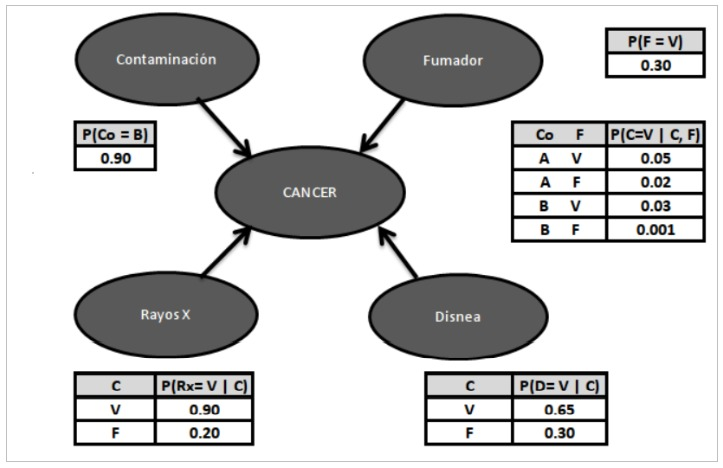
\includegraphics[width=3.32292in,height=\textheight]{images/WhatsApp Image 2023-05-26 at 21.19.34.jpeg}

}

\caption{Fig 1. Ejemplo de Redes Bayesianas}

\end{figure}

\hypertarget{redes-bayesianas-dinamicas}{%
\subsection{Redes Bayesianas
Dinamicas}\label{redes-bayesianas-dinamicas}}

Se han modificado a lo largo del tiempo. De esta forma se tiene una red
bayesiana que en cada instante de tiempo recibe infromacion del instante
anterior, ademas de las variables observables. En principio, representan
el estado de las variables en un cierto momento en el tiempo.

\hypertarget{refrencias-bibliograficas}{%
\subsubsection{REFRENCIAS
BIBLIOGRAFICAS}\label{refrencias-bibliograficas}}

\begin{itemize}
\item
  Rojas, J. C. S., Pérez, D. U., \& Reyes, C. E. H. (2012, junio 21).
  Definición de Redes Bayesianas y sus aplicaciones. Revista Vinculando.
  https://vinculando.org/articulos/redes-bayesianas.html
\item
  Introducción a la inferencia Bayesiana con Python. (2017).
  https://relopezbriega.github.io/blog/2017/05/21/introduccion-a-la-inferencia-bayesiana-con-python/
\item
  \emph{Inteligencia Artificial Redes bayesianas}. (s/f).
  Slideshare.net. Recuperado el 21 de mayo de 2023, de
  https://es.slideshare.net/hmartinezc2/inteligencia-artificial-redes-bayesianas
\end{itemize}



\end{document}
